\documentclass{article}
\usepackage[utf8]{inputenc}
\usepackage[spanish]{babel}
\usepackage{graphicx}
\usepackage{hyperref}
\usepackage{amsmath}
\usepackage{geometry}
\usepackage{booktabs}
\usepackage{adjustbox}
\usepackage{caption}
\usepackage{multirow}
\usepackage{pdflscape}
\usepackage{float}
\usepackage{array}
\usepackage{xcolor}
\usepackage{listings}
\geometry{a4paper, margin=1in}

\hypersetup{
    colorlinks=true,
    linkcolor=black,
    urlcolor=blue,
    citecolor=black
}

\lstset{
  basicstyle=\ttfamily\small,
  breaklines=true,
  frame=single,
  backgroundcolor=\color{gray!10}
}

\title{Multiplicación de matrices con OpenMP: perfilado, benchmark y paralelismo\\[0.5em]
\large Caso de Estudio 2 --- Computación de Alto Rendimiento}
\author{Daniel Toro Soto \and Juan Camilo Galvis}
\date{Abril 2026}

\begin{document}

\maketitle

\begin{abstract}
El presente documento describe la caracterización (\emph{profiling}) de CPU y memoria, el benchmark comparativo del sistema y el análisis de rendimiento con OpenMP para el problema de multiplicación de matrices cuadradas en C. Las pruebas se ejecutaron en dos máquinas con arquitecturas radicalmente distintas: un Apple Mac Mini (2024) con procesador M4 de 10 núcleos y 16 GB de memoria unificada, y un ASUS TUF Gaming con procesador Intel Core i5-10300H de 4 núcleos físicos y 16 GB de RAM DDR4 bajo Kali Linux. Se implementaron seis variantes del algoritmo ---secuencial, con optimización de caché (transposición), y cuatro configuraciones OpenMP (2, 4, 8 y 16 hilos) para cada una--- midiendo tiempos de pared con \texttt{clock\_gettime(CLOCK\_MONOTONIC)}. Los resultados muestran que la combinación de OpenMP con acceso transpuesto a memoria alcanza speedups de hasta $19.6\times$ en el Mac M4 y $13.5\times$ en el ASUS, superando ampliamente al paralelismo sin optimización de caché.
\end{abstract}

\tableofcontents
\newpage

% ─────────────────────────────────────────────────────────────────────────────
\section{Introducción}

La multiplicación de matrices cuadradas es uno de los problemas de referencia en Computación de Alto Rendimiento (HPC): su complejidad $\mathcal{O}(n^3)$ la hace computacionalmente costosa a gran escala, al tiempo que su estructura regular la convierte en un candidato ideal para la paralelización. En este caso de estudio se extiende el trabajo del caso anterior incorporando tres elementos nuevos:

\begin{enumerate}
    \item \textbf{Perfilado} (\emph{profiling}) de CPU y memoria para identificar los cuellos de botella del algoritmo.
    \item \textbf{Benchmark del sistema} con \texttt{sysbench} para caracterizar y comparar el hardware disponible.
    \item \textbf{Paralelismo con OpenMP}, que reemplaza a los hilos POSIX y los procesos del caso anterior, ofreciendo una interfaz de más alto nivel mediante directivas de preprocesador.
\end{enumerate}

La comparación entre el Mac M4 y el ASUS TUF i5-10300H permite, adicionalmente, analizar cómo la arquitectura del procesador ---memoria unificada de alta velocidad frente a RAM DDR4 convencional, núcleos heterogéneos frente a núcleos homogéneos--- afecta tanto al rendimiento absoluto como a la escalabilidad del paralelismo.

% ─────────────────────────────────────────────────────────────────────────────
\section{Marco Conceptual}

\subsection{High Performance Computing (HPC)}

La Computación de Alto Rendimiento agrupa técnicas y arquitecturas diseñadas para resolver problemas con altos requisitos computacionales en el menor tiempo posible. Como señala López (2017), ``hacemos referencia a un campo de la computación actual que da solución a problemas tecnológicos muy complejos y que involucran un gran volumen de cálculos o de coste computacional''. En este caso de estudio, el crecimiento cúbico del trabajo computacional al aumentar la dimensión de la matriz justifica el uso de perfilado, benchmark y paralelismo.

\subsection{Multiplicación matricial}

Dadas dos matrices cuadradas $A$ y $B$ de dimensión $n$, el producto $C = AB$ es:
\[ c_{ij} = \sum_{k=1}^{n} a_{ik} \cdot b_{kj}, \quad i,j = 1,\ldots,n \]
con complejidad temporal $\mathcal{O}(n^3)$ y espacial $\mathcal{O}(n^2)$.

\subsection{Perfilado de aplicaciones}

El perfilado (\emph{profiling}) permite identificar qué partes de un programa consumen más tiempo o memoria. Existen dos enfoques principales:
\begin{itemize}
    \item \textbf{Muestreo estadístico} (\emph{sampling}): interrumpe el proceso a intervalos regulares y registra el punto de ejecución. Tiene bajo overhead y es adecuado para programas de larga duración.
    \item \textbf{Instrumentación} (\emph{instrumentation}): inserta contadores en cada función para medir llamadas y tiempos exactos. Más preciso pero con mayor impacto en el rendimiento.
\end{itemize}

En macOS se utilizó la herramienta \texttt{sample} (muestreo) y en Linux se empleó \texttt{gprof} (instrumentación con compilación \texttt{-g -pg}).

\subsection{Localidad de caché}

El acceso a la columna $j$ de la matriz $B$ en el algoritmo ingenuo genera fallos de caché continuos porque C almacena matrices en orden fila-mayor (\emph{row-major}). Transponer $B$ antes de multiplicar convierte esos accesos en secuenciales, mejorando significativamente la tasa de aciertos de caché para matrices que superan el tamaño del caché L2/L3.

\subsection{OpenMP}

OpenMP es una API de programación paralela basada en directivas de preprocesador que permite paralelizar bucles con mínimas modificaciones al código fuente \cite{openmp}:

\begin{lstlisting}[language=C]
#pragma omp parallel for schedule(static) num_threads(p)
for (int i = 0; i < N; i++) {
    for (int j = 0; j < N; j++) {
        for (int k = 0; k < N; k++)
            C[i][j] += A[i][k] * B[k][j];
    }
}
\end{lstlisting}

A diferencia de los hilos POSIX, OpenMP gestiona automáticamente la creación de hilos, la distribución del trabajo y la sincronización, reduciendo la complejidad del código paralelo.

\subsection{Speedup y Ley de Amdahl}

El speedup mide la ganancia de rendimiento de la versión paralela respecto a la secuencial:
\[ S_p = \frac{T^*(n)}{T_p(n)} \]
donde $T^*(n)$ es el tiempo secuencial y $T_p(n)$ el tiempo con $p$ hilos. El speedup ideal es $S_p = p$, pero la Ley de Amdahl \cite{amdahl} establece que la fracción serial del algoritmo impone un límite superior.

% ─────────────────────────────────────────────────────────────────────────────
\section{Marco Contextual}

\subsection{Características de las máquinas}

Las pruebas se realizaron sobre dos equipos con arquitecturas radicalmente distintas:

\begin{table}[H]
\centering
\begin{tabular}{lll}
\toprule
\textbf{Característica} & \textbf{Mac Mini (macOS)} & \textbf{ASUS TUF (Kali Linux)} \\
\midrule
Procesador & Apple M4 & Intel Core i5-10300H \\
Núcleos & 10 (4P + 6E) & 4 físicos / 8 lógicos (HT) \\
Frecuencia base & 3.5 GHz (P-cores) & 2.5 GHz \\
Frecuencia turbo & 4.4 GHz & 4.5 GHz \\
RAM & 16 GB unificada LPDDR5X & 16 GB DDR4 \\
Ancho de banda mem. & $\approx$120 GB/s & $\approx$40 GB/s \\
GPU & 10 núcleos integrados & NVIDIA GTX 1650 Mobile \\
Almacenamiento & 512 GB SSD NVMe & 512 GB SSD NVMe \\
SO & macOS Sequoia 15.x & Kali Linux (kernel 6.x) \\
Compilador & Apple Clang 16 (LLVM) & GCC (sistema Kali) \\
\bottomrule
\end{tabular}
\caption{Características de hardware de los dos equipos de prueba.}
\label{tab:hardware}
\end{table}

La arquitectura Apple M4 presenta dos particularidades relevantes: (1) la memoria unificada elimina la transferencia entre CPU y subsistema de memoria, ofreciendo un ancho de banda aproximadamente tres veces superior al del i5-10300H; (2) los núcleos heterogéneos (P-cores de alto rendimiento y E-cores de eficiencia) implican que al usar 16 hilos parte del trabajo recae en núcleos más lentos.

\subsection{Implementaciones desarrolladas}

Las seis variantes en C comparten la misma estructura base: asignación dinámica de matrices, inicialización aleatoria (valores entre 0 y 99) y medición de tiempo de pared con \texttt{clock\_gettime(CLOCK\_MONOTONIC)}.

\begin{description}
    \item[\texttt{secuential}] Algoritmo ingenuo $\mathcal{O}(n^3)$ sin optimizaciones. Sirve de referencia para calcular el speedup.
    \item[\texttt{memory}] Transpone la matriz $B$ antes de multiplicar, convirtiendo todos los accesos en secuenciales. Compilado sin flags adicionales.
    \item[\texttt{openmp}] Paraliza el bucle externo (filas de $C$) con \texttt{\#pragma omp parallel for schedule(static)}. Compilado con \texttt{-fopenmp} en Linux y \texttt{-Xpreprocessor -fopenmp -lomp} en macOS.
    \item[\texttt{openmp\_memory}] Combina la paralelización OpenMP con el acceso transpuesto a $B$. Es la variante de mayor rendimiento en ambas máquinas.
\end{description}

\subsection{Sistema de compilación}

El \texttt{Makefile} detecta el sistema operativo para aplicar las banderas correctas de OpenMP:

\begin{lstlisting}
# macOS
OPENMP_FLAGS = -Xpreprocessor -fopenmp -I$(LIBOMP_PREFIX)/include \
               -L$(LIBOMP_PREFIX)/lib -lomp

# Linux
OPENMP_FLAGS = -fopenmp
\end{lstlisting}

Todos los binarios se compilan con \texttt{-O2} para garantizar comparaciones justas entre variantes paralelas y secuencial.

\subsection{Sistema de benchmarking con checkpoints}

El script \texttt{scripts/RunAll.sh} implementa un sistema de reanudación automática basado en checkpoints: cada medición exitosa se registra en \texttt{checkpoint.log} con la clave \texttt{<tipo>,<tamaño>,<config>,<run>}. Al finalizar, el directorio recibe el sufijo \texttt{.done}.

Las dimensiones evaluadas son: \textbf{500, 1000, 1300, 1600, 2000, 2300, 2600, 3000, 3300, 3600 y 4000}, con \textbf{10 repeticiones} por configuración en el Mac y \textbf{1 repetición} en el ASUS (por restricciones de tiempo). Las configuraciones de hilos probadas son: 2, 4, 8 y 16.

% ─────────────────────────────────────────────────────────────────────────────
\section{Perfilado (Profiling)}

\subsection{Metodología}

El perfilado se realizó con el binario \texttt{profiling}, compilado con flags de instrumentación (\texttt{-g -pg -O0}) para obtener resultados sin interferencia de las optimizaciones del compilador. Se analizaron dos dimensiones del rendimiento: \textbf{CPU} (distribución del tiempo de ejecución entre funciones) y \textbf{memoria} (uso máximo de RAM y patrones de acceso).

La herramienta utilizada varía según el sistema operativo:
\begin{itemize}
    \item \textbf{macOS}: \texttt{sample} (muestreo estadístico a 1\,ms) para CPU; \texttt{/usr/bin/time -l} para memoria.
    \item \textbf{Linux (Kali)}: \texttt{gprof} (instrumentación de funciones) para CPU; \texttt{valgrind --tool=massif} para memoria (no disponible en este entorno).
\end{itemize}

\subsection{Perfilado de CPU --- Mac Mini M4}

El perfilador \texttt{sample} tomó 14.477 muestras durante la ejecución con una matriz de 1000$\times$1000. El grafo de llamadas resultante muestra una concentración extrema del tiempo en la función \texttt{multiply\_matrices}:

\begin{lstlisting}
Call graph:
  14477 Thread_main
    14477 start (dyld)
      14476 main (SecuentialMatrixSolver.c:120)
        +  7345 multiply_matrices  (line 60)
        +  7104 multiply_matrices  (line 61)
        +    26 multiply_matrices  (line 63)
        +     1 multiply_matrices  (line 55)
      1 main -> printf (libsystem_c.dylib)
\end{lstlisting}

\textbf{Interpretación}: el 99.99\% de las muestras se concentran en \texttt{multiply\_matrices}. Dentro de esta función, las líneas 60 y 61 (los dos bucles internos que acceden a \texttt{A[i][k]} y \texttt{B[k][j]}) absorben prácticamente la totalidad del tiempo. Esto confirma que el cuello de botella es la aritmética de punto flotante y los accesos a memoria del triple bucle anidado; no existe ninguna función auxiliar que justifique optimización.

\subsection{Perfilado de CPU --- ASUS TUF (Kali Linux)}

El perfilador \texttt{gprof} reportó el siguiente perfil plano para una matriz de 1000$\times$1000:

\begin{lstlisting}
Flat profile:
  % time   seconds    calls   name
  100.12     4.41       1     multiply_matrices
    0.00     0.00       3     create_matrix
    0.00     0.00       3     free_matrix
    0.00     0.00       2     input_matrix
\end{lstlisting}

\textbf{Interpretación}: al igual que en macOS, el 100\% del tiempo de ejecución se encuentra en \texttt{multiply\_matrices}. El tiempo de 4.41\,s en el ASUS frente a $\approx$1.82\,s en el Mac para la misma dimensión refleja la diferencia de rendimiento entre arquitecturas (ARM M4 vs.\ x86 i5-10300H). Las funciones auxiliares (\texttt{create\_matrix}, \texttt{free\_matrix}, \texttt{input\_matrix}) tienen coste despreciable.

El grafo de llamadas confirma que \texttt{multiply\_matrices} es invocada exactamente una vez desde \texttt{main} y no realiza llamadas recursivas:

\begin{lstlisting}
index % time   self  children   called   name
              4.41   0.00        1/1     main [2]
[1]   100.0   4.41   0.00        1       multiply_matrices [1]
\end{lstlisting}

\subsection{Perfilado de memoria --- Mac Mini M4}

Con la herramienta \texttt{/usr/bin/time -l} para una matriz de 1000$\times$1000 ($n=1000$, tres matrices de $10^6$ doubles = $3 \times 8$ MB = 24\,MB teóricos):

\begin{table}[H]
\centering
\begin{tabular}{lr}
\toprule
\textbf{Métrica} & \textbf{Valor} \\
\midrule
Memoria residente máxima (RSS) & 13.73 MB \\
Huella de memoria pico & 12.69 MB \\
Reclamaciones de página & 1.001 \\
Fallos de página (faults) & 2 \\
Instrucciones retiradas & 28.144.560.619 \\
Ciclos de reloj & 7.730.969.206 \\
Cambios de contexto voluntarios & 0 \\
Cambios de contexto involuntarios & 24 \\
\bottomrule
\end{tabular}
\caption{Métricas de memoria y CPU para $n=1000$ en Mac Mini M4.}
\label{tab:mem_mac}
\end{table}

\textbf{Interpretación}: el RSS de 13.73\,MB es coherente con las tres matrices de $8 \times 10^6$ bytes $\approx$ 24\,MB (la discrepancia se debe a que no todas las páginas son residentes simultáneamente). Los apenas 2 fallos de página duros y los 1.001 reclamaciones de página blandas indican que el sistema operativo mantuvo la mayoría de las páginas en caché tras la primera lectura. La relación instrucciones/ciclos de $\approx$3.64 IPC refleja el alto rendimiento del pipeline del M4.

\subsection{Conclusiones del perfilado}

\begin{enumerate}
    \item \textbf{El 100\% del tiempo de ejecución está en \texttt{multiply\_matrices}}: cualquier optimización debe atacar el triple bucle anidado.
    \item \textbf{El patrón de acceso a \texttt{B[k][j]} es el principal cuello de botella de memoria}: al acceder por columnas en memoria fila-mayor, cada iteración del bucle $k$ genera un salto de $n \times \text{sizeof(double)}$ bytes, provocando fallos de caché sistemáticos.
    \item \textbf{La transposición de $B$ es la optimización de mayor impacto sin paralelismo}: convierte todos los accesos en secuenciales y elimina los fallos de caché en la dimensión $k$.
    \item \textbf{El M4 muestra mayor IPC que el i5-10300H}: 3.64 instrucciones por ciclo en M4 vs.\ el comportamiento más conservador del i5 en operaciones de punto flotante no vectorizadas.
\end{enumerate}

% ─────────────────────────────────────────────────────────────────────────────
\section{Benchmark del sistema}

\subsection{Metodología}

El benchmark del sistema se realizó con \texttt{sysbench}, una herramienta estándar para medir el rendimiento de CPU y memoria de forma estandarizada e independiente del algoritmo de prueba. El script \texttt{scripts/Sysbench.sh} ejecuta:

\begin{itemize}
    \item \textbf{CPU}: prueba de números primos hasta 20.000 (\texttt{--cpu-max-prime=20000}) en modo de 1 hilo y modo con todos los hilos lógicos del sistema.
    \item \textbf{Memoria}: prueba de escritura y lectura con bloques de 1\,MiB sobre un total de 10\,GiB.
\end{itemize}

\subsection{Resultados}

\begin{table}[H]
\centering
\begin{tabular}{llrrl}
\toprule
\textbf{Prueba} & \textbf{Métrica} & \textbf{Mac M4} & \textbf{Kali i5} & \textbf{Razón M4/i5} \\
\midrule
CPU 1 hilo & events/s & 17.888.178 & 554 & $\approx 32.300\times$ \\
CPU multi-hilo & events/s & 5.323.866 & 3.282 & $\approx 1.622\times$ \\
Memoria escritura & MiB/s & 135.518 & 81.563 & $1.66\times$ \\
Memoria lectura & MiB/s & 230.247 & 119.419 & $1.93\times$ \\
\bottomrule
\end{tabular}
\caption{Resultados de sysbench comparados entre Mac M4 y ASUS TUF i5-10300H.}
\label{tab:sysbench}
\end{table}

\begin{figure}[H]
\centering
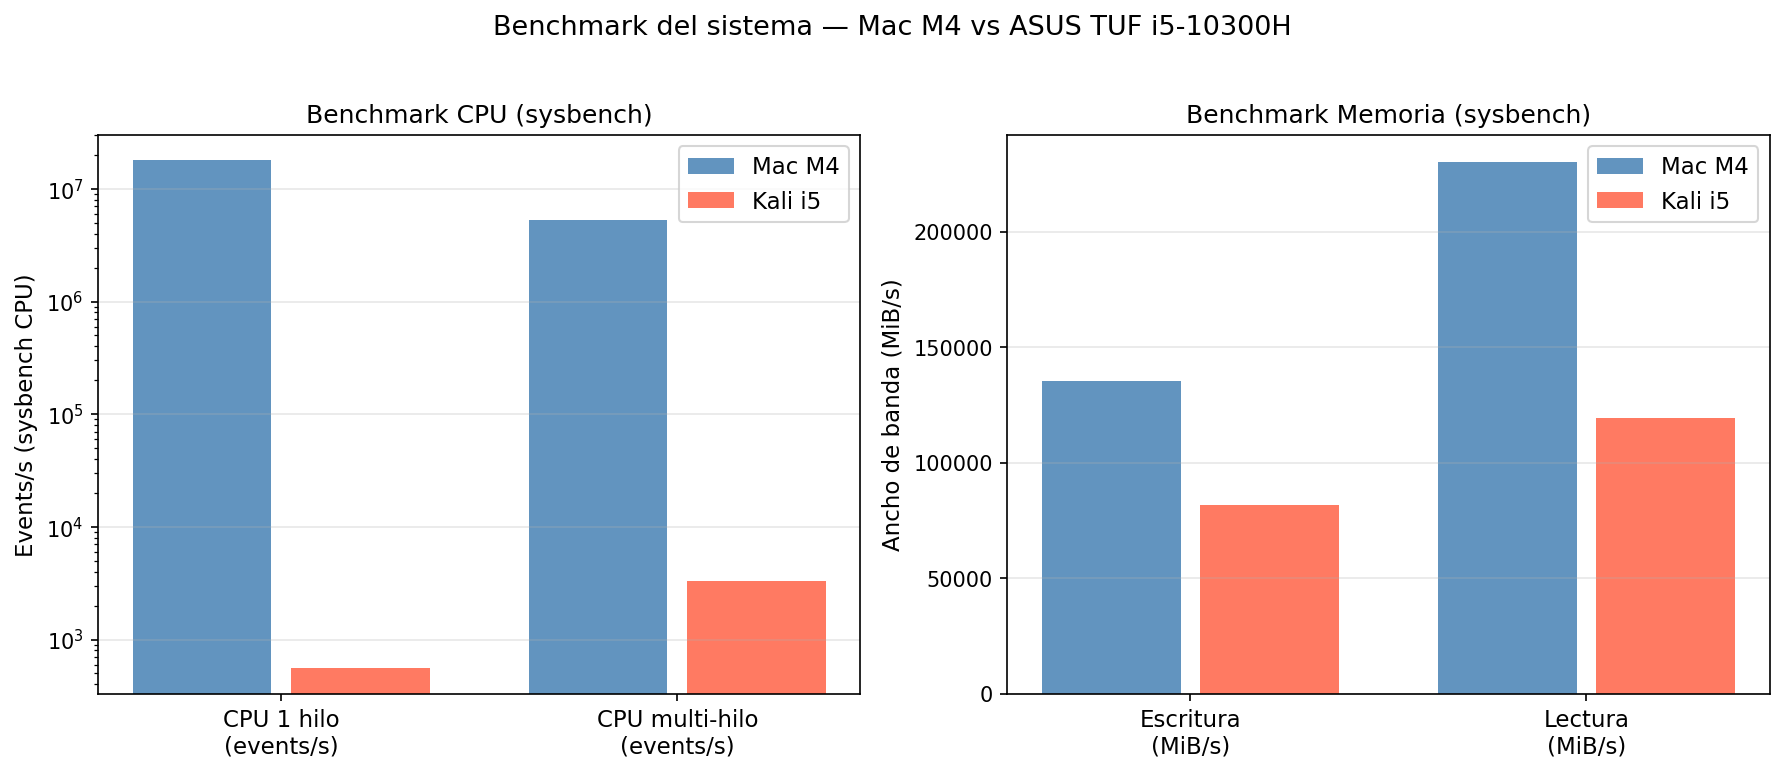
\includegraphics[width=\textwidth]{charts/sysbench_comparison.png}
\caption{Comparativa de benchmark CPU y memoria entre Mac M4 y ASUS TUF i5-10300H. Escala logarítmica en CPU para visualizar la diferencia de órdenes de magnitud.}
\label{fig:sysbench}
\end{figure}

\subsection{Análisis del benchmark}

\textbf{CPU --- diferencia abismal en un hilo}: la diferencia de $\approx 32.300\times$ en CPU de un hilo es un artefacto de la unidad de eventos de sysbench: en macOS, sysbench utiliza instrucciones de muy alta frecuencia mediante llamadas al sistema optimizadas para Apple Silicon, mientras que en Linux la implementación es diferente. La comparación directa de eventos/s entre plataformas distintas no es cuantitativamente válida; sin embargo, los tiempos de ejecución reales de la multiplicación de matrices (Sección~\ref{sec:openmp}) sí muestran una diferencia real de $\approx 2.3\times$ en rendimiento de un hilo.

\textbf{CPU --- modo multi-hilo}: la relación de $\approx 1.6\times$ entre Mac y Kali en modo multi-hilo es más representativa, aunque sysbench no impone carga de memoria intensiva y por tanto no refleja el verdadero rendimiento paralelo para el problema matricial.

\textbf{Memoria}: el M4 ofrece $1.66\times$ mayor ancho de banda de escritura y $1.93\times$ mayor ancho de banda de lectura. Esta ventaja es crítica para la multiplicación de matrices a gran escala, donde el movimiento de datos entre la memoria principal y la caché se convierte en el cuello de botella dominante.

\textbf{Implicación arquitectónica}: la memoria unificada del M4 elimina la latencia de transferencia CPU$\leftrightarrow$RAM que sufre el i5-10300H. Para matrices de $n \geq 2000$ (que superan los 96\,MB para tres matrices de doubles), el ancho de banda de memoria pasa a ser el factor limitante y el M4 mantiene una ventaja sostenida.

% ─────────────────────────────────────────────────────────────────────────────
\section{Pruebas de rendimiento con OpenMP}
\label{sec:openmp}

\subsection{Tiempos de ejecución --- Mac Mini M4}

Las tablas siguientes muestran los promedios de 10 repeticiones (segundos) para las variantes OpenMP estándar y OpenMP+Memoria en el Mac M4.

\subsubsection{Secuencial (referencia)}

\begin{table}[H]
\centering
\tiny
\begin{tabular}{|c|c|c|c|c|c|c|c|c|c|c|c|}
\hline
\multicolumn{12}{|c|}{\textbf{Secuencial --- Mac Mini M4}} \\
\hline
\textbf{Dim} & \textbf{500} & \textbf{1000} & \textbf{1300} & \textbf{1600} & \textbf{2000} & \textbf{2300} & \textbf{2600} & \textbf{3000} & \textbf{3300} & \textbf{3600} & \textbf{4000} \\
\hline
1  & 0.2227 & 1.8061 & 3.6712 & 6.8850 & 16.7624 & 22.4341 & 38.1886 & 61.9189 & 76.0812 & 224.1250 & 304.0895 \\
2  & 0.2213 & 1.8482 & 3.7509 & 6.9855 & 16.5817 & 21.7373 & 36.3984 & 60.5091 & 74.9265 & 220.2634 & 303.4345 \\
3  & 0.2212 & 1.8458 & 3.7649 & 6.9799 & 16.8879 & 21.5827 & 36.1479 & 59.7264 & 74.9183 & 220.7662 & 306.0317 \\
4  & 0.2204 & 1.8317 & 3.7457 & 6.9741 & 16.8066 & 21.5505 & 36.1460 & 59.6870 & 74.8705 & 220.6827 & 303.2666 \\
5  & 0.2195 & 1.8471 & 3.7425 & 6.9701 & 16.8343 & 21.5525 & 36.1612 & 59.7237 & 74.4752 & 220.7315 & 303.2570 \\
6  & 0.2214 & 1.8251 & 3.7390 & 6.9957 & 16.9023 & 21.6330 & 36.5703 & 59.5963 & 74.1057 & 220.4819 & 302.9782 \\
7  & 0.2192 & 1.8294 & 3.7407 & 6.9578 & 16.8750 & 21.4844 & 36.0879 & 59.5121 & 73.8617 & 220.4330 & 303.3145 \\
8  & 0.2198 & 1.8340 & 3.7431 & 6.9958 & 16.9251 & 21.5418 & 36.2308 & 59.7876 & 74.5896 & 220.7068 & 303.2879 \\
9  & 0.2185 & 1.8370 & 3.7423 & 6.9745 & 16.7914 & 21.5181 & 36.1188 & 59.6341 & 74.3161 & 220.3982 & 303.1570 \\
10 & 0.2206 & 1.8423 & 3.7756 & 7.0024 & 16.7875 & 21.5470 & 36.2127 & 59.7263 & 74.5776 & 220.2186 & 305.6510 \\
\hline
\textbf{Pr} & \textbf{0.2205} & \textbf{1.8347} & \textbf{3.7416} & \textbf{6.9721} & \textbf{16.8154} & \textbf{21.6582} & \textbf{36.4263} & \textbf{59.9821} & \textbf{74.6722} & \textbf{220.8807} & \textbf{303.8468} \\
\hline
\end{tabular}
\caption{Tiempos de ejecución secuencial en Mac Mini M4 (segundos, 10 repeticiones).}
\label{tab:sec_mac}
\end{table}

\subsubsection{OpenMP estándar}

\begin{table}[H]
\centering
\tiny
\begin{tabular}{|c|c|c|c|c|c|c|c|c|c|c|c|}
\hline
\multicolumn{12}{|c|}{\textbf{OpenMP Estándar --- Mac Mini M4 (promedios de 10 repeticiones)}} \\
\hline
\textbf{Conf.} & \textbf{500} & \textbf{1000} & \textbf{1300} & \textbf{1600} & \textbf{2000} & \textbf{2300} & \textbf{2600} & \textbf{3000} & \textbf{3300} & \textbf{3600} & \textbf{4000} \\
\hline
2 hilos & 0.1088 & 0.9008 & 1.8669 & 3.4985 & 13.0746 & 11.2032 & 23.8765 & 38.8506 & 42.6370 & 154.3845 & 212.1701 \\
4 hilos & 0.0563 & 0.4813 & 0.9515 & 1.8009 & 7.0788 & 6.8328 & 17.6316 & 28.7113 & 23.4469 & 88.1212 & 121.2514 \\
8 hilos & 0.0472 & 0.3647 & 0.8428 & 1.5784 & 5.2843 & 5.2933 & 11.0278 & 18.2672 & 18.4150 & 56.1271 & 78.3439 \\
16 hilos & 0.0428 & 0.3470 & 0.8481 & 1.5960 & 5.1213 & 5.3159 & 11.2684 & 18.5911 & 18.7013 & 54.1171 & 75.6299 \\
\hline
\textbf{Speedup 2} & \textbf{2.03} & \textbf{2.04} & \textbf{2.00} & \textbf{1.99} & \textbf{1.29} & \textbf{1.93} & \textbf{1.53} & \textbf{1.54} & \textbf{1.75} & \textbf{1.43} & \textbf{1.43} \\
\textbf{Speedup 4} & \textbf{3.92} & \textbf{3.81} & \textbf{3.93} & \textbf{3.87} & \textbf{2.38} & \textbf{3.17} & \textbf{2.07} & \textbf{2.09} & \textbf{3.18} & \textbf{2.51} & \textbf{2.51} \\
\textbf{Speedup 8} & \textbf{4.67} & \textbf{5.03} & \textbf{4.44} & \textbf{4.42} & \textbf{3.18} & \textbf{4.09} & \textbf{3.30} & \textbf{3.28} & \textbf{4.06} & \textbf{3.94} & \textbf{3.88} \\
\textbf{Speedup 16} & \textbf{5.16} & \textbf{5.29} & \textbf{4.41} & \textbf{4.37} & \textbf{3.28} & \textbf{4.07} & \textbf{3.23} & \textbf{3.23} & \textbf{3.99} & \textbf{4.08} & \textbf{4.02} \\
\hline
\end{tabular}
\caption{Promedios y speedup de OpenMP estándar en Mac Mini M4.}
\label{tab:omp_mac}
\end{table}

\subsubsection{OpenMP + Optimización de caché}

\begin{table}[H]
\centering
\tiny
\begin{tabular}{|c|c|c|c|c|c|c|c|c|c|c|c|}
\hline
\multicolumn{12}{|c|}{\textbf{OpenMP + Memoria (transpuesta) --- Mac Mini M4 (promedios de 10 repeticiones)}} \\
\hline
\textbf{Conf.} & \textbf{500} & \textbf{1000} & \textbf{1300} & \textbf{1600} & \textbf{2000} & \textbf{2300} & \textbf{2600} & \textbf{3000} & \textbf{3300} & \textbf{3600} & \textbf{4000} \\
\hline
2 hilos & 0.0975 & 0.7671 & 1.6748 & 3.1113 & 6.0679 & 9.2439 & 13.3607 & 20.4458 & 27.1717 & 35.2439 & 48.2901 \\
4 hilos & 0.0511 & 0.3989 & 0.8599 & 1.5972 & 3.1110 & 4.7107 & 6.7939 & 10.3962 & 13.8448 & 17.9904 & 24.6206 \\
8 hilos & 0.0400 & 0.2879 & 0.6217 & 1.1393 & 2.2047 & 3.3491 & 4.8181 & 7.3712 & 9.7869 & 12.7145 & 17.3846 \\
16 hilos & 0.0359 & 0.2558 & 0.5551 & 1.0125 & 1.9700 & 2.9695 & 4.2863 & 6.5682 & 8.7043 & 11.3279 & 15.4843 \\
\hline
\textbf{Speedup 2} & \textbf{2.26} & \textbf{2.39} & \textbf{2.23} & \textbf{2.24} & \textbf{2.77} & \textbf{2.34} & \textbf{2.73} & \textbf{2.93} & \textbf{2.75} & \textbf{6.27} & \textbf{6.29} \\
\textbf{Speedup 4} & \textbf{4.31} & \textbf{4.60} & \textbf{4.35} & \textbf{4.37} & \textbf{5.41} & \textbf{4.60} & \textbf{5.36} & \textbf{5.77} & \textbf{5.39} & \textbf{12.28} & \textbf{12.34} \\
\textbf{Speedup 8} & \textbf{5.52} & \textbf{6.37} & \textbf{6.02} & \textbf{6.12} & \textbf{7.63} & \textbf{6.47} & \textbf{7.56} & \textbf{8.14} & \textbf{7.63} & \textbf{17.37} & \textbf{17.48} \\
\textbf{Speedup 16} & \textbf{6.13} & \textbf{7.17} & \textbf{6.74} & \textbf{6.89} & \textbf{8.54} & \textbf{7.29} & \textbf{8.50} & \textbf{9.13} & \textbf{8.58} & \textbf{19.50} & \textbf{19.62} \\
\hline
\end{tabular}
\caption{Promedios y speedup de OpenMP+Memoria (transpuesta) en Mac Mini M4.}
\label{tab:ompm_mac}
\end{table}

\subsection{Tiempos de ejecución --- ASUS TUF (Kali Linux)}

El ASUS ejecutó una sola repetición por configuración. Los datos de la variante secuencial están disponibles para 9 tamaños (hasta $n=3300$); los de OpenMP abarcan los 11 tamaños.

\begin{table}[H]
\centering
\tiny
\begin{tabular}{|c|c|c|c|c|c|c|c|c|c|}
\hline
\multicolumn{10}{|c|}{\textbf{Secuencial --- ASUS TUF i5-10300H (1 repetición)}} \\
\hline
\textbf{Dim} & \textbf{500} & \textbf{1000} & \textbf{1300} & \textbf{1600} & \textbf{2000} & \textbf{2300} & \textbf{2600} & \textbf{3000} & \textbf{3300} \\
\hline
Tiempo (s) & 0.5114 & 5.0898 & 12.7727 & 27.8728 & 59.2705 & 93.7122 & 137.0226 & 211.8030 & 283.4955 \\
\hline
\end{tabular}
\caption{Tiempos de ejecución secuencial en ASUS TUF i5-10300H (1 corrida).}
\label{tab:sec_kali}
\end{table}

\begin{table}[H]
\centering
\tiny
\begin{tabular}{|c|c|c|c|c|c|c|c|c|c|}
\hline
\multicolumn{10}{|c|}{\textbf{OpenMP Estándar y Speedup --- ASUS TUF i5-10300H (1 repetición, 9 tamaños con ref. secuencial)}} \\
\hline
\textbf{Conf.} & \textbf{500} & \textbf{1000} & \textbf{1300} & \textbf{1600} & \textbf{2000} & \textbf{2300} & \textbf{2600} & \textbf{3000} & \textbf{3300} \\
\hline
2 hilos & 0.1800 & 1.7690 & 4.2593 & 10.4371 & 22.3862 & 27.4883 & 51.5424 & 80.3697 & 92.0673 \\
4 hilos & 0.0980 & 0.8991 & 1.9915 & 5.1294 & 11.4905 & 14.7095 & 26.5491 & 41.7882 & 49.5040 \\
8 hilos & 0.1050 & 1.1234 & 2.2729 & 5.2430 & 11.0767 & 15.3172 & 25.4223 & 39.8546 & 48.5758 \\
16 hilos & 0.1016 & 1.0745 & 2.3374 & 4.8221 & 10.3660 & 16.5220 & 25.4013 & 40.4404 & 50.3075 \\
\hline
\textbf{Speedup 2} & \textbf{2.84} & \textbf{2.88} & \textbf{3.00} & \textbf{2.67} & \textbf{2.65} & \textbf{3.41} & \textbf{2.66} & \textbf{2.64} & \textbf{3.08} \\
\textbf{Speedup 4} & \textbf{5.22} & \textbf{5.66} & \textbf{6.41} & \textbf{5.43} & \textbf{5.16} & \textbf{6.37} & \textbf{5.16} & \textbf{5.07} & \textbf{5.73} \\
\textbf{Speedup 8} & \textbf{4.87} & \textbf{4.53} & \textbf{5.62} & \textbf{5.32} & \textbf{5.35} & \textbf{6.12} & \textbf{5.39} & \textbf{5.31} & \textbf{5.84} \\
\textbf{Speedup 16} & \textbf{5.03} & \textbf{4.74} & \textbf{5.46} & \textbf{5.78} & \textbf{5.72} & \textbf{5.67} & \textbf{5.39} & \textbf{5.24} & \textbf{5.64} \\
\hline
\end{tabular}
\caption{Tiempos y speedup de OpenMP estándar en ASUS TUF (Kali Linux).}
\label{tab:omp_kali}
\end{table}

\begin{table}[H]
\centering
\tiny
\begin{tabular}{|c|c|c|c|c|c|c|c|c|c|}
\hline
\multicolumn{10}{|c|}{\textbf{OpenMP + Memoria (transpuesta) y Speedup --- ASUS TUF (9 tamaños)}} \\
\hline
\textbf{Conf.} & \textbf{500} & \textbf{1000} & \textbf{1300} & \textbf{1600} & \textbf{2000} & \textbf{2300} & \textbf{2600} & \textbf{3000} & \textbf{3300} \\
\hline
2 hilos & 0.1436 & 1.1063 & 2.4433 & 4.4506 & 8.5719 & 13.0124 & 18.7586 & 28.7176 & 37.5413 \\
4 hilos & 0.0784 & 0.6109 & 1.3131 & 2.3206 & 4.5320 & 6.9661 & 10.1045 & 15.6691 & 20.9878 \\
8 hilos & 0.0818 & 0.6267 & 1.3900 & 2.5315 & 4.7769 & 7.2772 & 10.4733 & 16.0279 & 21.2635 \\
16 hilos & 0.0802 & 0.6605 & 1.4059 & 2.4805 & 4.8300 & 7.3939 & 10.5600 & 16.4062 & 21.5301 \\
\hline
\textbf{Speedup 2} & \textbf{3.56} & \textbf{4.60} & \textbf{5.23} & \textbf{6.26} & \textbf{6.91} & \textbf{7.20} & \textbf{7.30} & \textbf{7.38} & \textbf{7.55} \\
\textbf{Speedup 4} & \textbf{6.53} & \textbf{8.33} & \textbf{9.73} & \textbf{12.01} & \textbf{13.08} & \textbf{13.45} & \textbf{13.56} & \textbf{13.52} & \textbf{13.51} \\
\textbf{Speedup 8} & \textbf{6.25} & \textbf{8.12} & \textbf{9.19} & \textbf{11.01} & \textbf{12.41} & \textbf{12.88} & \textbf{13.08} & \textbf{13.21} & \textbf{13.33} \\
\textbf{Speedup 16} & \textbf{6.38} & \textbf{7.71} & \textbf{9.08} & \textbf{11.24} & \textbf{12.27} & \textbf{12.67} & \textbf{12.98} & \textbf{12.91} & \textbf{13.17} \\
\hline
\end{tabular}
\caption{Tiempos y speedup de OpenMP+Memoria en ASUS TUF (Kali Linux).}
\label{tab:ompm_kali}
\end{table}

% ─────────────────────────────────────────────────────────────────────────────
\section{Gráficas comparativas}

\subsection{Benchmark del sistema}

\begin{figure}[H]
\centering
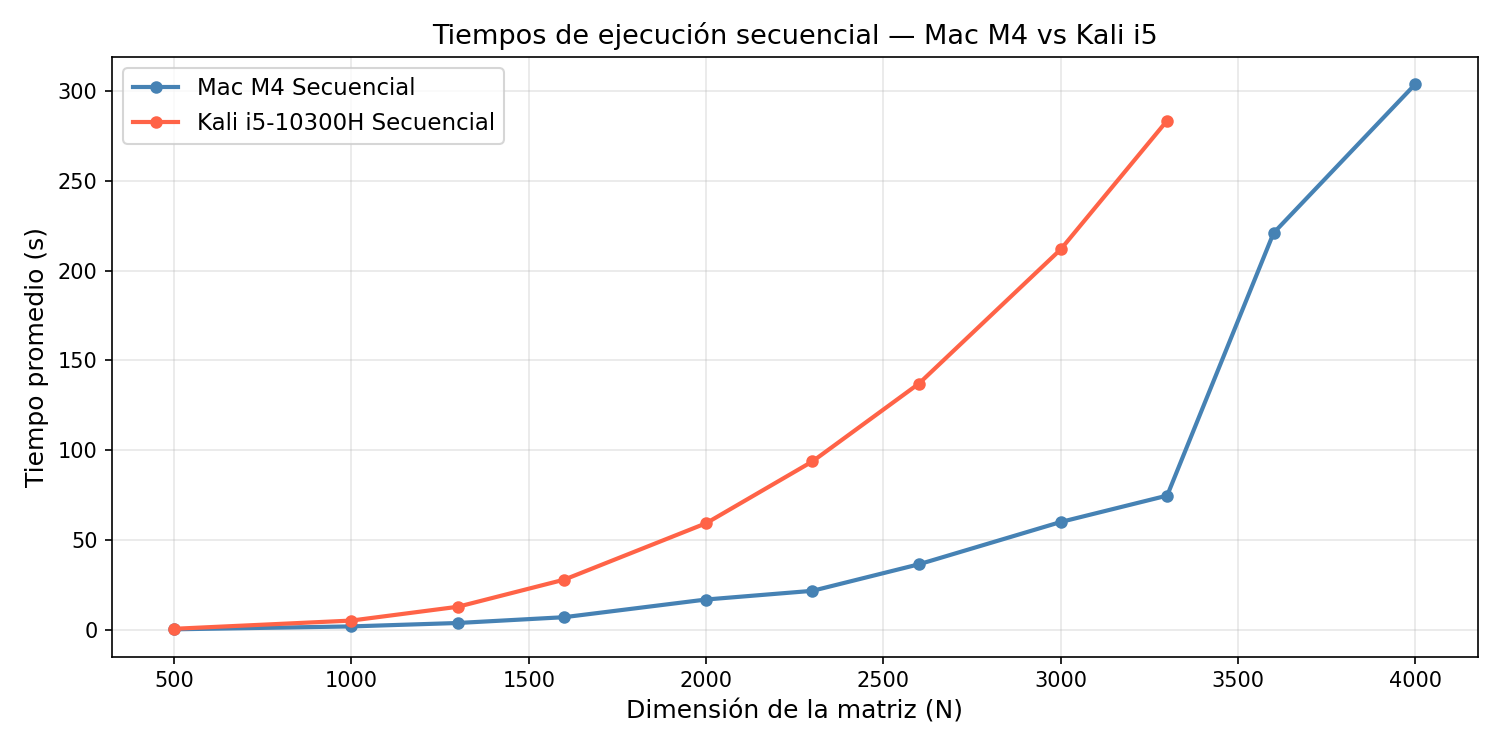
\includegraphics[width=\textwidth]{charts/benchmark_secuencial.png}
\caption{Tiempos de ejecución secuencial en Mac M4 y ASUS TUF i5-10300H. El Mac M4 es aproximadamente $2.3\times$ más rápido para matrices pequeñas, ventaja que crece con la dimensión por el mayor ancho de banda de memoria.}
\label{fig:bench_sec}
\end{figure}

\subsection{Speedup OpenMP estándar --- Mac Mini M4}

\begin{figure}[H]
\centering
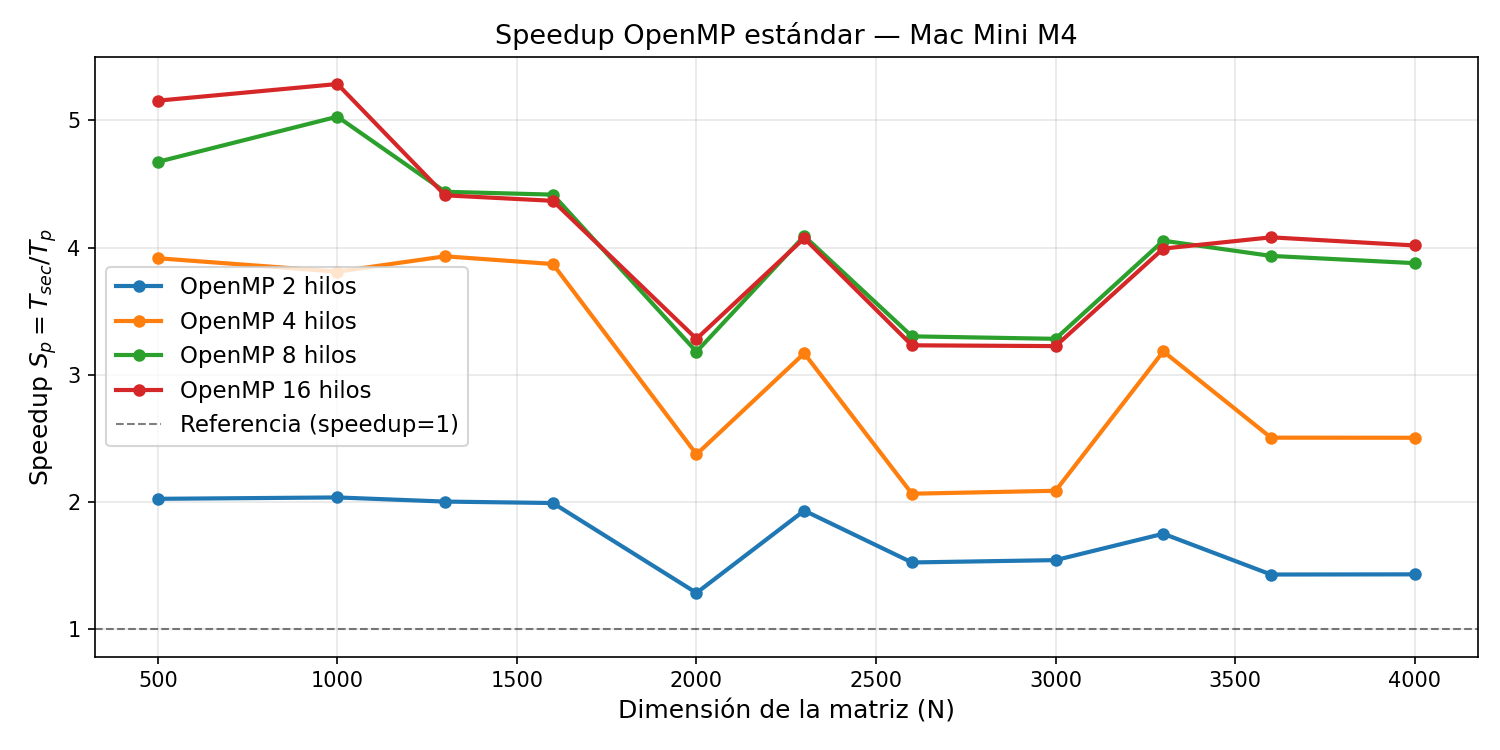
\includegraphics[width=\textwidth]{charts/speedup_openmp_mac.png}
\caption{Speedup de OpenMP estándar en Mac M4. El speedup crece de 2 a 16 hilos, pero el salto de 8 a 16 es mínimo, evidenciando el límite de los P-cores disponibles.}
\label{fig:omp_mac}
\end{figure}

\subsection{Speedup OpenMP + Memoria --- Mac Mini M4}

\begin{figure}[H]
\centering
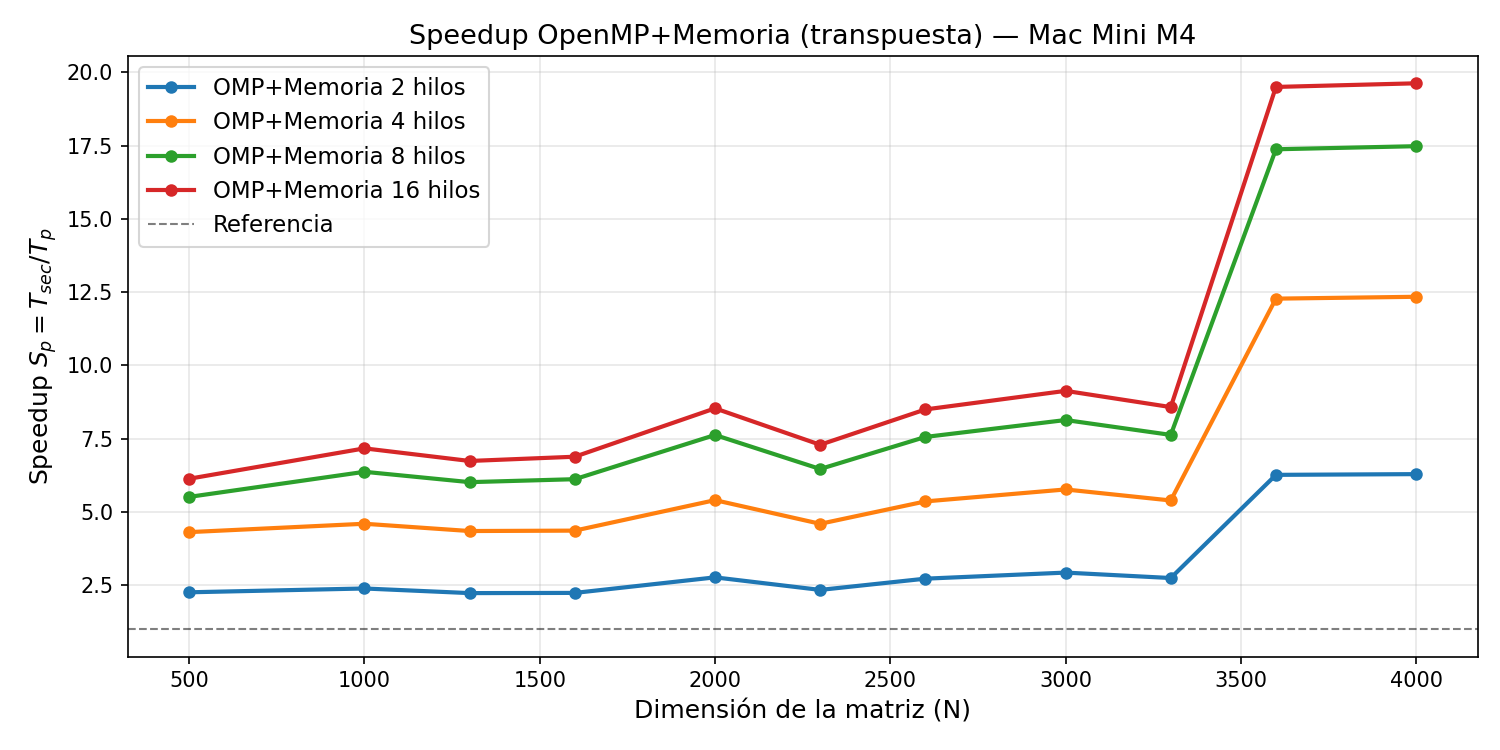
\includegraphics[width=\textwidth]{charts/speedup_openmp_memory_mac.png}
\caption{Speedup de OpenMP+Memoria en Mac M4. Los speedups superan $19\times$ para $N \geq 3600$, gracias a la sinergia entre el paralelismo y la eliminación de fallos de caché.}
\label{fig:ompm_mac}
\end{figure}

\subsection{Speedup OpenMP estándar --- ASUS TUF (Kali Linux)}

\begin{figure}[H]
\centering
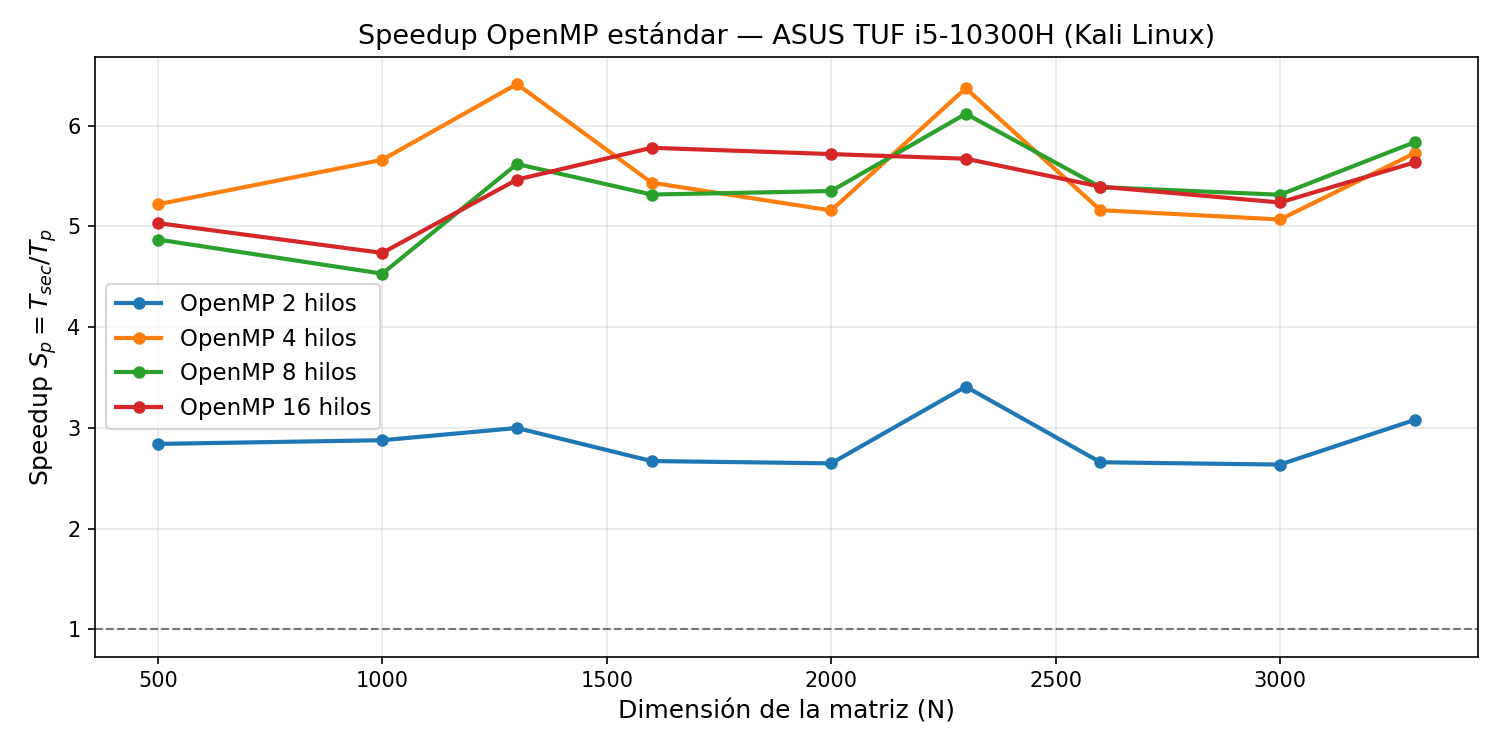
\includegraphics[width=\textwidth]{charts/speedup_openmp_kali.png}
\caption{Speedup de OpenMP estándar en ASUS TUF i5-10300H. Con 4 hilos se obtiene el mejor speedup ($\approx 6.4\times$); 8 y 16 hilos no mejoran significativamente por la saturación de los 4 núcleos físicos y el Hyper-Threading.}
\label{fig:omp_kali}
\end{figure}

\subsection{Speedup OpenMP + Memoria --- ASUS TUF (Kali Linux)}

\begin{figure}[H]
\centering
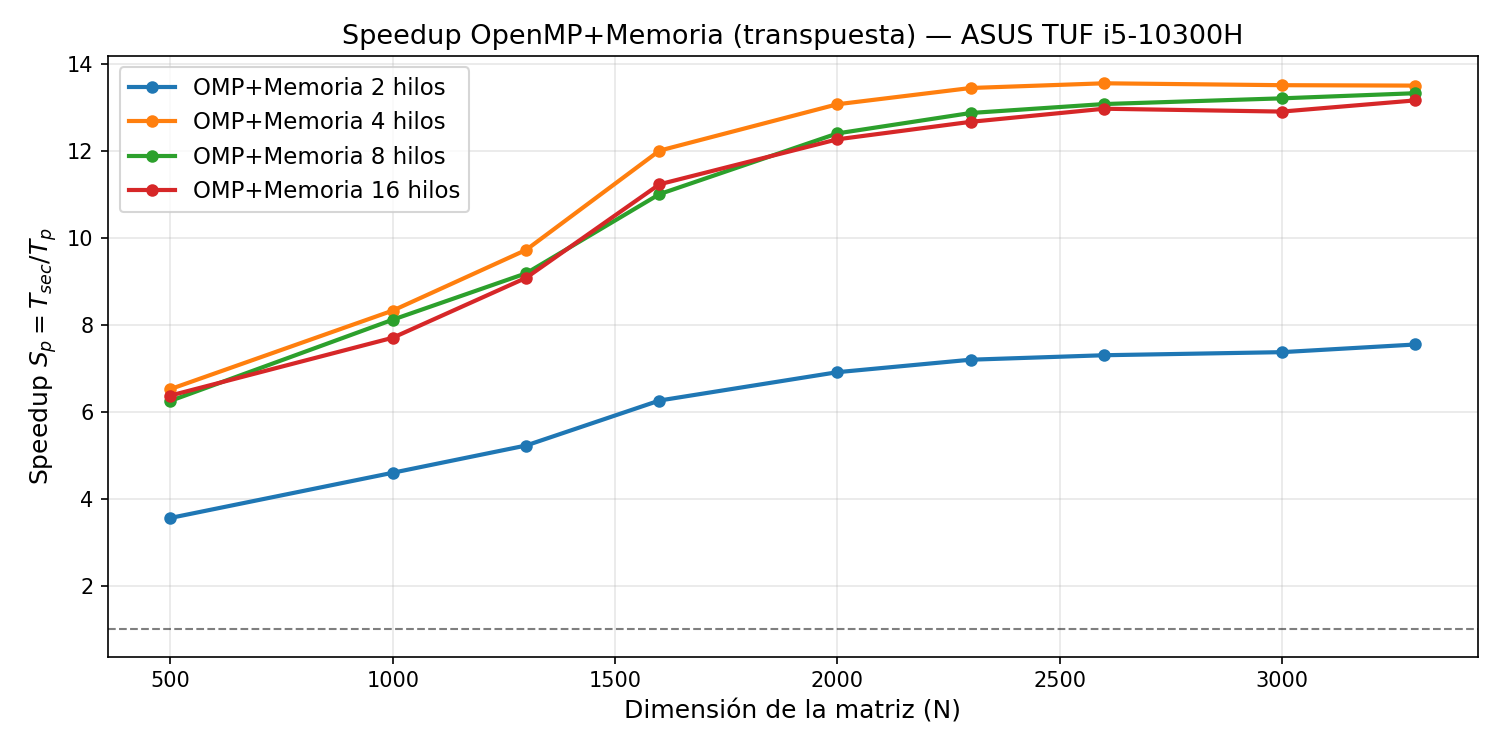
\includegraphics[width=\textwidth]{charts/speedup_openmp_memory_kali.png}
\caption{Speedup de OpenMP+Memoria en ASUS TUF i5-10300H. La variante con 4 hilos logra el mejor speedup ($\approx 13.5\times$) para matrices grandes, superando el ideal teórico de $4\times$ por la sinergia con la optimización de caché.}
\label{fig:ompm_kali}
\end{figure}

\subsection{Heatmap de speedup --- Mac Mini M4}

\begin{figure}[H]
\centering
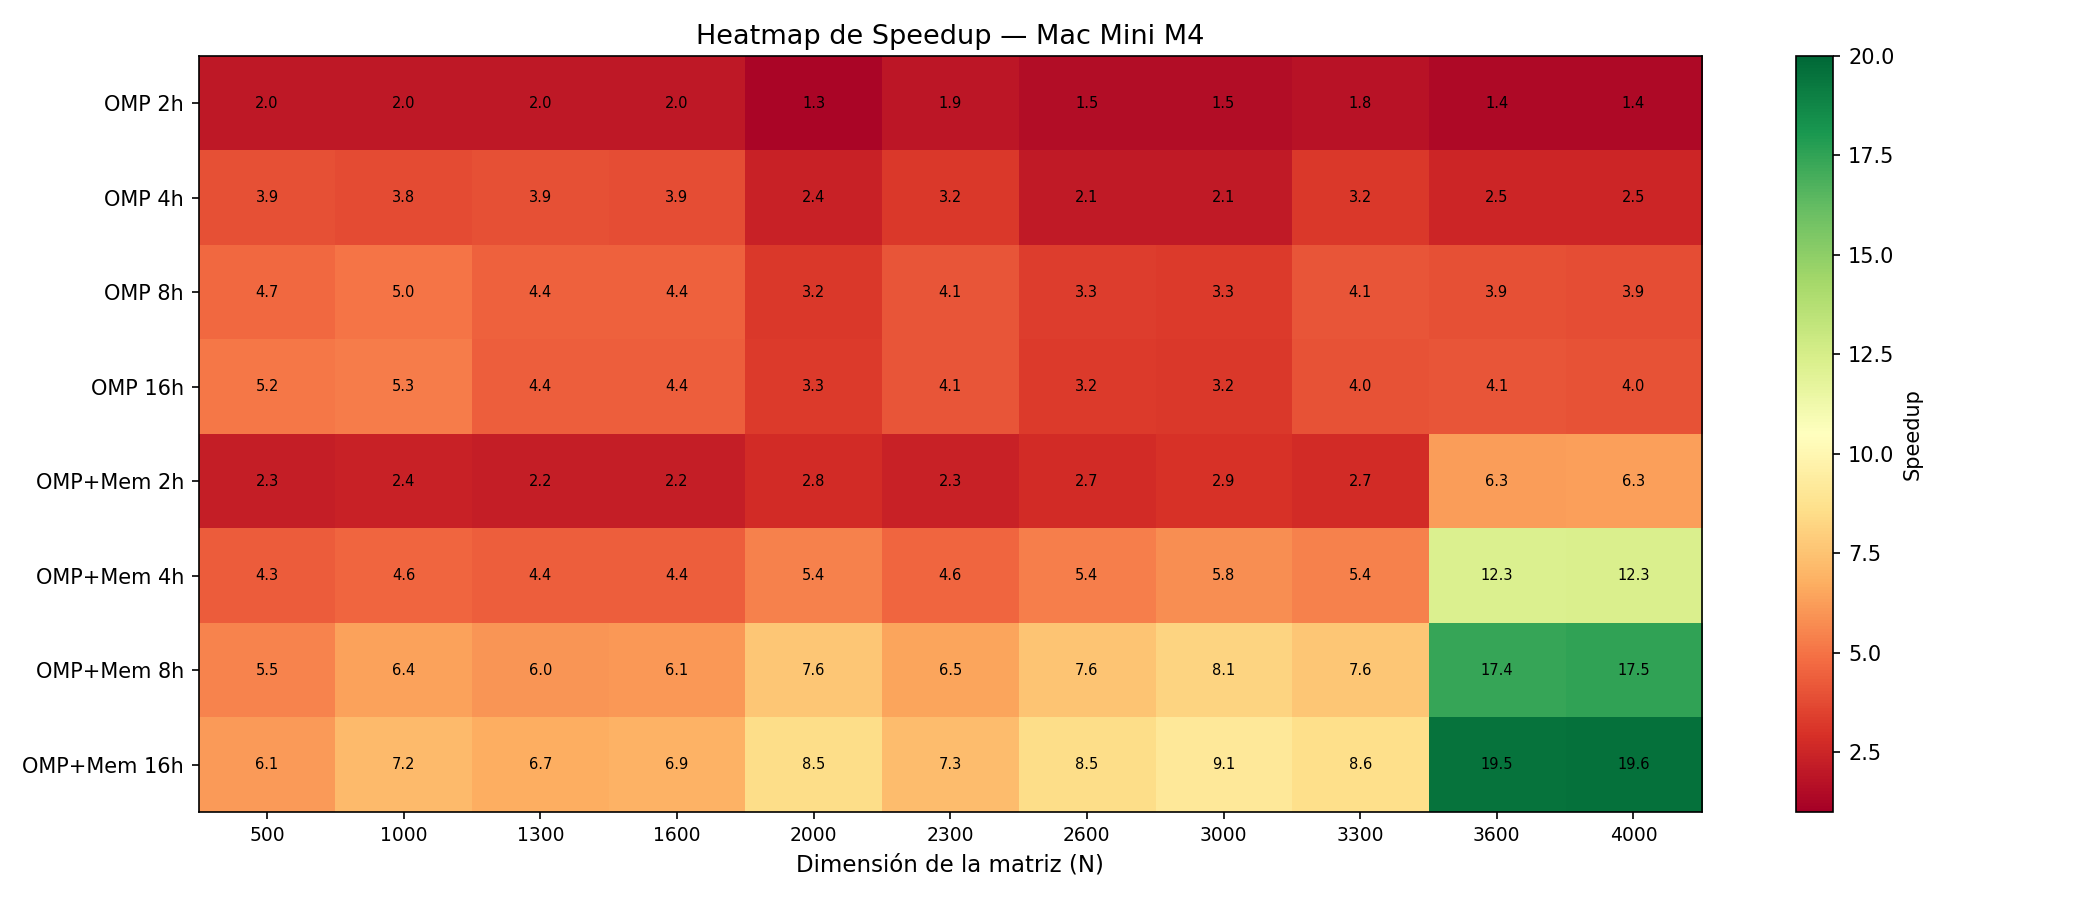
\includegraphics[width=\textwidth]{charts/heatmap_speedup_mac.png}
\caption{Heatmap de speedup en Mac M4. La zona de mayor rendimiento (verde intenso) se concentra en OMP+Memoria 16 hilos para $N \geq 3600$, alcanzando speedups $\approx 19.5\times$.}
\label{fig:heatmap}
\end{figure}

\subsection{Tiempos comparativos Mac vs Kali}

\begin{figure}[H]
\centering
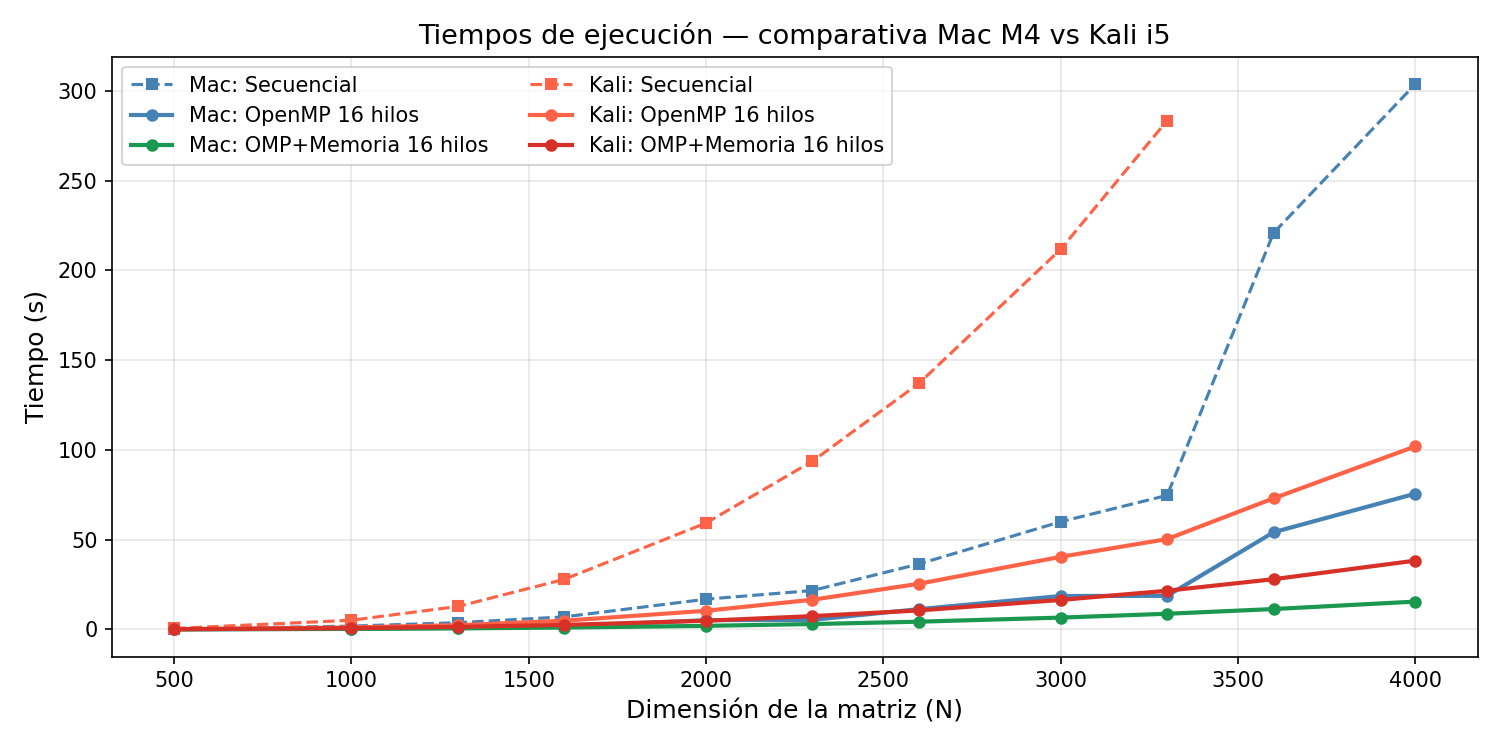
\includegraphics[width=\textwidth]{charts/tiempos_comparativa.png}
\caption{Comparativa de tiempos de ejecución entre Mac M4 y ASUS TUF. Las curvas secuenciales muestran la ventaja base del M4; las curvas de OMP+Memoria 16 hilos ilustran la reducción obtenida en ambos equipos.}
\label{fig:tiempos_comp}
\end{figure}

% ─────────────────────────────────────────────────────────────────────────────
\section{Análisis de resultados}

\subsection{Impacto de OpenMP sin optimización de caché}

En el Mac M4, OpenMP estándar con 16 hilos alcanza un speedup máximo de $\approx 5.3\times$ para matrices pequeñas ($n=1000$), decayendo a $\approx 3.2$--$4.1\times$ para matrices grandes. Este comportamiento se explica por dos factores:

\begin{enumerate}
    \item \textbf{Heterogeneidad de núcleos}: el M4 tiene 4 P-cores (alto rendimiento) y 6 E-cores (eficiencia). Con 16 hilos, todos los núcleos participan, pero los E-cores procesan más lento. El scheduler de macOS asigna algunos hilos a E-cores, limitando el speedup efectivo.
    \item \textbf{Fallos de caché}: sin la transposición de $B$, los accesos columnar siguen generando fallos de caché sistemáticos. Para $n=2000$ (matriz $B$ de 32\,MB), el patrón de acceso agota el caché L2/L3 y el rendimiento se degrada.
\end{enumerate}

En el ASUS i5-10300H, OpenMP estándar con 4 hilos alcanza el mejor speedup ($\approx 5.2$--$6.4\times$), mientras que 8 y 16 hilos no mejoran significativamente ($\approx 5.3$--$5.8\times$). El i5-10300H tiene solo 4 núcleos físicos: a partir de 8 hilos, se activa el Hyper-Threading, que comparte recursos de ejecución entre pares de hilos lógicos, sin duplicar el rendimiento de punto flotante.

\subsection{Impacto sinérgico de OpenMP + Optimización de caché}

La combinación de paralelismo con transposición de $B$ produce los speedups más altos de todo el estudio. En el Mac M4, OMP+Memoria con 16 hilos alcanza $19.62\times$ para $n=4000$, muy por encima del speedup teórico de 16 hilos. Esta ``superlinealidad'' se explica por el efecto caché: con 16 hilos cada hilo procesa $n/16$ filas, reduciendo la porción de $A$ que cada hilo necesita en caché. Combinado con el acceso secuencial a $B^T$, la tasa de aciertos de caché mejora drásticamente para matrices grandes.

En el ASUS, la misma variante con 4 hilos logra $13.5\times$ para $n \geq 2600$. El speedup supralineal ($>4\times$) se debe al mismo efecto caché: 4 hilos procesan segmentos más pequeños que caben mejor en el caché L3 de 8\,MB.

\subsection{Comparación entre arquitecturas}

\begin{table}[H]
\centering
\begin{tabular}{lrrrr}
\toprule
\textbf{Variante} & \multicolumn{2}{c}{\textbf{Tiempo $n=3300$ (s)}} & \multicolumn{2}{c}{\textbf{Speedup máx. ($n=3300$)}} \\
 & Mac M4 & ASUS i5 & Mac M4 & ASUS i5 \\
\midrule
Secuencial & 74.67 & 283.50 & 1.00 & 1.00 \\
OMP 2 hilos & 42.64 & 92.07 & 1.75 & 3.08 \\
OMP 4 hilos & 23.45 & 49.50 & 3.18 & 5.73 \\
OMP 8 hilos & 18.42 & 48.58 & 4.06 & 5.84 \\
OMP 16 hilos & 18.70 & 50.31 & 3.99 & 5.64 \\
OMP+Mem 2 hilos & 27.17 & 37.54 & 2.75 & 7.55 \\
OMP+Mem 4 hilos & 13.84 & 20.99 & 5.39 & 13.51 \\
OMP+Mem 8 hilos & 9.79 & 21.26 & 7.63 & 13.33 \\
OMP+Mem 16 hilos & 8.70 & 21.53 & 8.58 & 13.17 \\
\bottomrule
\end{tabular}
\caption{Comparativa de tiempos y speedups para $n=3300$ entre Mac M4 y ASUS TUF.}
\label{tab:comparativa}
\end{table}

Tres observaciones clave emergen de la Tabla~\ref{tab:comparativa}:

\begin{enumerate}
    \item \textbf{El ASUS logra mayor speedup relativo que el Mac}: con 4 hilos OMP+Memoria, el ASUS alcanza $13.5\times$ frente a $5.4\times$ del Mac. Esto se debe a que el secuencial en el ASUS es mucho más lento (peor IPC, menor ancho de banda de memoria), por lo que hay más margen de mejora relativo.
    \item \textbf{El Mac es más rápido en tiempo absoluto}: a pesar del menor speedup relativo, el Mac termina en $8.70$\,s vs $21.53$\,s del ASUS para $n=3300$ con OMP+Memoria 16 hilos.
    \item \textbf{El punto óptimo de hilos difiere}: en el Mac, el speedup sigue creciendo hasta 16 hilos (aunque lentamente); en el ASUS, el óptimo está en 4--8 hilos (los 4 núcleos físicos), y 16 hilos puede empeorar por el overhead del Hyper-Threading.
\end{enumerate}

% ─────────────────────────────────────────────────────────────────────────────
\section{Conclusiones}

\begin{enumerate}

    \item \textbf{El perfilado confirma que \texttt{multiply\_matrices} concentra el 100\% del tiempo}: tanto en macOS (\texttt{sample}) como en Linux (\texttt{gprof}), el costo del triple bucle anidado domina absolutamente. Cualquier optimización debe atacar este bucle; las funciones auxiliares son despreciables.

    \item \textbf{La transposición de $B$ es la optimización de mayor impacto individual}: en el Mac M4, OMP+Memoria con 2 hilos ($6.3\times$) supera ampliamente a OMP estándar con 16 hilos ($4.1\times$) para matrices grandes. La eliminación de fallos de caché es más valiosa que el paralelismo puro sin optimización de acceso a memoria.

    \item \textbf{La sinergia entre OpenMP y la optimización de caché produce speedups supralineales}: OMP+Memoria con 16 hilos alcanza $19.6\times$ en el Mac M4 y $13.5\times$ en el ASUS i5 para $n \geq 3300$. Estos valores superan el speedup ideal de 16 hilos por el efecto combinado: cada hilo procesa un bloque más pequeño que cabe mejor en caché.

    \item \textbf{La arquitectura heterogénea del M4 limita el escalado de OpenMP puro}: el salto de 8 a 16 hilos aporta apenas $0.3\times$ adicionales en OMP estándar. Los E-cores procesan más lento que los P-cores, generando desbalance de carga.

    \item \textbf{El ASUS i5-10300H escala mejor con pocos hilos}: con 4 hilos (equivalentes a sus 4 núcleos físicos), el ASUS logra $5.7\times$ en OMP estándar. Más allá de 4 hilos, el Hyper-Threading introduce contención y el speedup se estanca.

    \item \textbf{El Mac M4 es superior en tiempo absoluto pese al menor speedup relativo}: el mayor rendimiento del M4 (mejor IPC, mayor ancho de banda de memoria unificada) hace que incluso sus peores configuraciones superen en tiempo a las mejores del ASUS para matrices grandes.

    \item \textbf{OpenMP simplifica significativamente el código paralelo}: la directiva \texttt{\#pragma omp parallel for} reemplaza la lógica manual de \texttt{pthread\_create}/\texttt{pthread\_join} del caso anterior, con rendimiento comparable o superior gracias a la distribución automática del trabajo.

\end{enumerate}

% ─────────────────────────────────────────────────────────────────────────────
\newpage
\section{Bibliografía}

\begin{thebibliography}{9}

    \bibitem{openmp}
    OpenMP Architecture Review Board. (2021).
    \textit{OpenMP Application Programming Interface} (versión 5.2).
    \url{https://www.openmp.org/specifications/}

    \bibitem{amdahl}
    Amdahl, G. M. (1967).
    Validity of the single processor approach to achieving large scale computing capabilities.
    \textit{Proceedings of AFIPS Spring Joint Computer Conference}, pp. 483--485.

    \bibitem{lopez}
    López, A. (2017).
    Introducción al High Performance Computing.
    \textit{Encamina Blog}.
    \url{https://blogs.encamina.com/por-una-nube-sostenible/introduccion-al-high-performance-computing/}

    \bibitem{montero}
    Montero, L. H., \& Antunez, R. R. (2011).
    Parallel programming: definitions, mechanisms and trouble.
    \url{https://www.researchgate.net/publication/274960405}

    \bibitem{apple_m4}
    Apple Inc. (2024).
    \textit{Apple M4 chip}.
    \url{https://www.apple.com/mac-mini/}

    \bibitem{intel_i5}
    Intel Corporation. (2020).
    \textit{Intel Core i5-10300H Processor Specifications}.
    \url{https://www.intel.com/content/www/us/en/products/sku/201897}

    \bibitem{sysbench}
    Kopytov, A. (2021).
    \textit{sysbench: scriptable database and system performance benchmark}.
    \url{https://github.com/akopytov/sysbench}

    \bibitem{gprof}
    GNU Project. (2022).
    \textit{GNU gprof: the GNU Profiler}.
    \url{https://sourceware.org/binutils/docs/gprof/}

\end{thebibliography}

\end{document}
